\documentclass{article}
\usepackage[utf8]{inputenc}
\usepackage[german]{babel}
\usepackage{graphicx} 
\usepackage{amsmath, amssymb}

\usepackage[square,numbers]{natbib}
\bibliographystyle{abbrvnat}

\title{Aufbau und Justage eines Leckstrahlmikroskopes zum Nachweis des plasmonischen Spin-Hall-Effektes}
\author{Hanno Christiansen}
\date{März 2021}

\begin{document}
	
\maketitle
\tableofcontents

\section{Einführung}
\section{Theorie}
	\subsection{Oberflächen-Plasmon-Polariton (SPP)}		
	Ein Oberflächen-Plasmon-Polariton (engl. Surface-Plasmon-Polariton SPP) ist das quantisierte Quasiteilchen, der an das elektromagnetischen Feld gekoppelten Elektronen-Dichte-Oszillation, an einer Dielektrikums-Metall-Grenzschicht. Durch die spezielle Form dieser Geometrie, ist es möglich, trotz des rein longitudinalen Charakters der Elektronen-Dichte-Oszillation, ein elektromagnetisches Feld mit transversalen Komponenten zu erzeugen. Diese transversalen Komponenten sind notwendig, damit eine Kopplung an das rein transversale elektromagnetische Feld des Vakuums tendenziell zu ermöglichen. Die einfachste Geometrie in der SPPs auftreten können ist ein Zwei-Schichtsystem. Der Halbraum oberhalb der $xy$-Ebene mit $z>0$ sei von einem Dielektrikum mit der Dielektrizitätskonstante $\epsilon_D"$ ausgefüllt. Der Halbraum unterhalb der $xy$-Ebene mit $z<0$ sei von einem Metall mit der im allgemeinen komplexen Dielektrischen-Funktion $\epsilon(\omega)$ ausgefüllt. An der Grenzschicht zwischen diesen beiden Halbräumen können SPPs propagieren. Um nun einige Charakteristische Eigenschaften von SPPs zu erläutern, gehe ich davon aus, dass das SPP entlang der $x$-Achse propagiert und entlang der y-Achse homogen ist. So wird das Problem effektiv 2-dimensional. Wie in \cite{Maier.2007} gezeigt, lassen sich die elektromagnetischen Felder eines SPPs in dieser einfachen Geometrie durch folgende Ausdrücke beschreiben:
	\begin{equation}
		\label{eq:electric_field_spp}
		\vec{E}_n = \begin{pmatrix} 1 \\ 0 \\ \pm k_{\mathrm{spp}}/k_{z,n} \end{pmatrix} E_0 \exp\left(i(k_{\mathrm{spp}}x + k_{z, n}|z|-\omega t)\right)	
	\end{equation}
	\begin{equation}
		\label{eq:magnetic_field_spp}
		\vec{H}_n = \begin{pmatrix} 0 \\ 1 \\ 0 \end{pmatrix} H_0 \exp\left(i(k_{\mathrm{spp}}x + k_{z, n}|z|-\omega t)\right)
	\end{equation}
	Der Index $n$ beschreibt hierbei das Material($M$ für das Metall, $D$ für das Dielektrikum). Das $\pm$ ist $+$ für das Metall und  $-$ für das Dielektrikum. $\omega$ ist die Winkelfrequenz der Anregung. $k_{\mathrm{spp}}$ ist der im allgemeinen komplexe Wellenvektor der Anregung.  $k_{\mathrm{spp}}$ ist für beide Medien gleich. Der Realteil $\operatorname{\mathbb{R}e}\{k_{\mathrm{spp}}\}$ des komplexen Wellenvektors lässt sich in die Wellenlänge $\lambda_{\mathrm{spp}} = 2\pi/ \operatorname{\mathbb{R}e}\{k_{\mathrm{spp}}\} $ des SPP umrechnen. Der Imaginärteil $\operatorname{\mathbb{I}m}\{k_{\mathrm{spp}}\}$ beschreibt das Dämpfungsverhalten des SPP entlang der Ausbreitungsrichtung. Es lässt sich über $\L_{\mathrm{spp}} = 1/(2\operatorname{\mathbb{I}m}\{k_{\mathrm{spp}}\})$ eine Propagationslänge definieren. Nachdem das SPP eine Propagationslänge zurückgelegt hat, sind die ursprünglichen Intensitäten des SPP auf $1/\mathrm{e}$ ihres ursprünglichen Betrages zurückgegangen.
	
	Analog beschreibt $\operatorname{\mathbb{R}e}\{k_{z, n}\}$ den Exponentiellen-Abfall der Anregung, wenn man sich von der Grenzfläche entfernt. Hier lassen sich die Eindringtiefen $\delta_{M,D}$ definieren, die angeben nach welcher Entfernung in z-Richtung die ursprungliche Feldstärke auf $1/\mathrm{e}$ abgeklungen ist. Das SPP hat sowohl transversale, als auch longitudinale Komponenten des Elektrischen Feldes. Das magnetische Feld ist rein transversal. Daher spricht man auch von einer Transversal-Magnetischen Anregung (TM).
	Der quantitativer Verlauf des elektrischen Feldes für ein rein reelles $k_{\mathrm{spp}}$ und ein rein imaginäres $k_{z, n}$ ist in Abb. \ref{fig:electric_field_spp} dargestellt.
	\begin{figure}[htbp] 
		\centering
		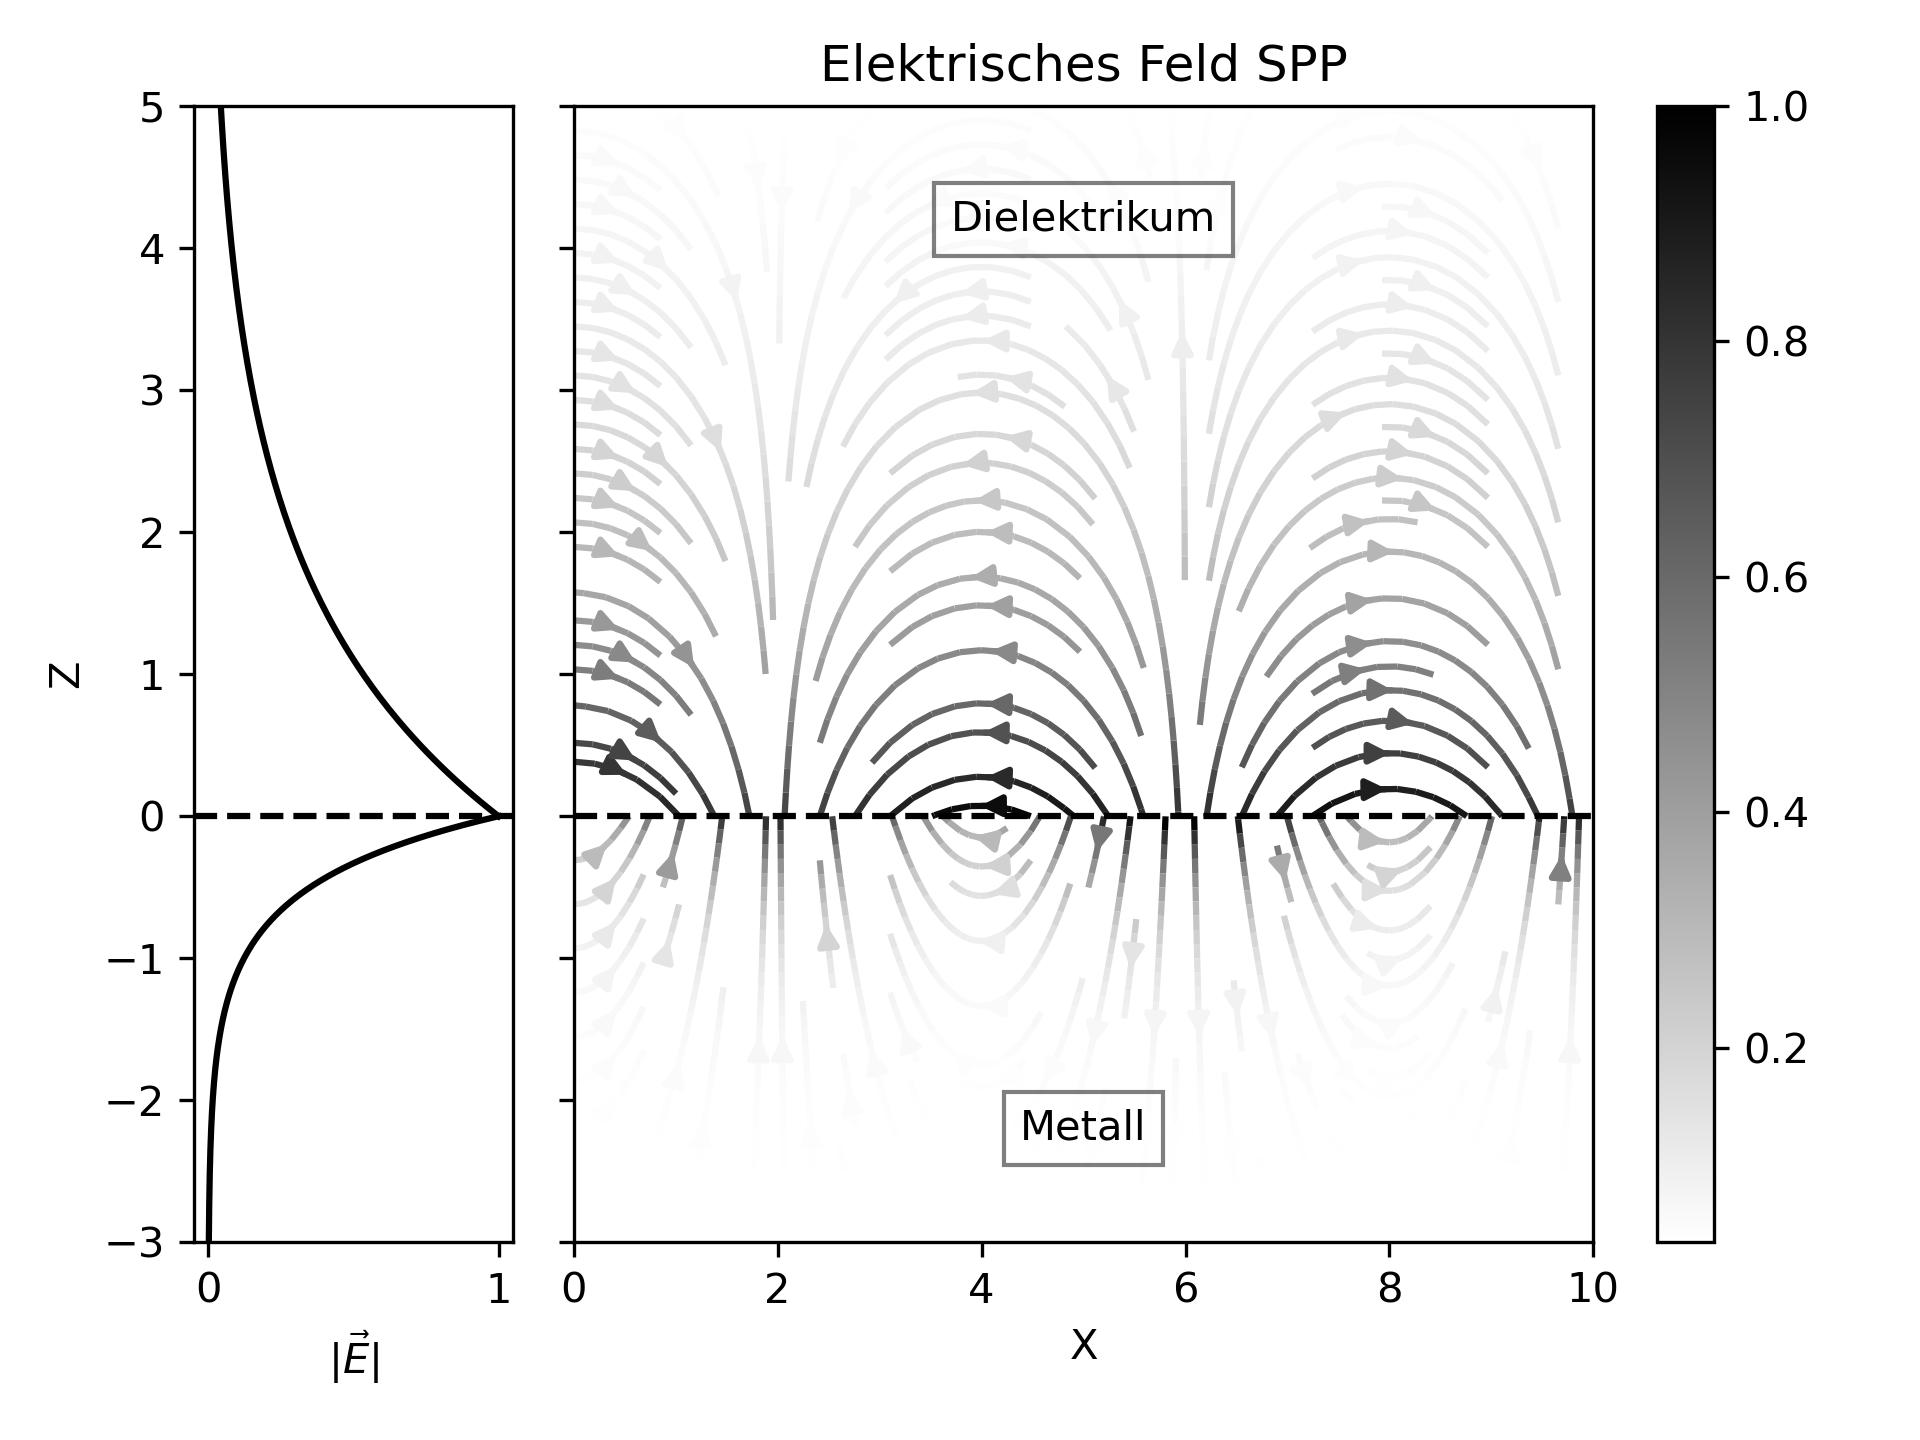
\includegraphics[width=1\textwidth]{figures/E_Feld_SPP.png}
		\caption{Quantitativer Verlauf des Elektrischen Feldes eines SPPs entlang einer Metall-Dielektrikums-Grenzschicht in der  xy-Ebene mit Ausbreitungsrichtung in positiver x-Richtung}
		\label{fig:electric_field_spp}
	\end{figure}

	\subsubsection{Dispersion}
	Die Herleitung der Dispersionsrelation orientiert sich an den Ausführungen in \cite[pp.~261--ff]{Fox.2020} und kann dort im Detail nachvollzogen werden. Ich beschränke mich hier auf eine kurze Beschreibung des Vorgehens.
	Damit die oben angesetzten elektromagnetischen Felder \eqref{eq:electric_field_spp}, \eqref{eq:magnetic_field_spp}  die Maxwellgleichungen \eqref{eq:maxwell} und die Randbedingungen an der Grenzschicht erfüllen, müssen die Bedingungen \eqref{eq:condition_spp_1},  \eqref{eq:condition_spp_2} gelten. (Hierbei handelt es sich um den Spezialfall nicht magnetischer Materialien.)
	\begin{align}
		\label{eq:maxwell}	
		&\vec{\nabla}\cdot\vec{D} = 0		&\vec{\nabla}\cdot\vec{B} = 0 \\
		&\vec{\nabla}\times\vec{E} = -\dfrac{\partial\vec{B}}{\partial t} 
		&\vec{\nabla}\times\vec{H} = 	\dfrac{\partial\vec{D}}{\partial t}\nonumber
	\end{align}
	\begin{subequations}
		\begin{equation}
			\label{eq:condition_spp_1}
			\dfrac{k_{z, M}}{\epsilon_M} + \dfrac{k_{z, D}}{\epsilon_D} = 0
		\end{equation}		
		\begin{equation}
			\label{eq:condition_spp_2}
			k_{\mathrm{spp}}^2 +k_{z, n}^2 = \epsilon_n\left(\dfrac{\omega}{c}\right)^2; \text{ für  } n=M,D
		\end{equation}
		\end{subequations}
		$\epsilon_{M, D} = \epsilon_{M, D}(\omega) $ sind hierbei die Permittivitäten der Materialien in Abhängigkeit von der Kreisfrequenz. Aus Gleichung \eqref{eq:condition_spp_2} folgt $k_{z, n} = \sqrt{\epsilon_n k_0^2 - k_{\mathrm{spp}}^2}$. Diese Beziehung legt den Zusammenhang zwischen $k_{\mathrm{spp}}$ und $k_{z, n}$ fest. Außerdem lässt sich hieraus erkennen, dass für typische Materialien $ \operatorname{\mathbb{I}m}\{k_{z, n}\} \gg \operatorname{\mathbb{R}e}\{k_{z, n}\}$. Durch die Dominanz des Imaginärteils über den Realteil der Wellenvektorkomponente senkrecht zur Ausbreitungsrichtung, fallen die Felder senkrecht zu Ausbreitungsrichtung exponentiell ab. Man spricht deswegen von evaneszenten Feldern. Die Anregung ist daher stark an die Grenzfläche gebunden. Durch das Lösen der Bedingungen \eqref{eq:condition_spp_1},  \eqref{eq:condition_spp_2} ergibt sich die Dispersionsrelation des SPP an einer Grenzschicht zwischen einem Metall und einem Dielektrikum zu: 
	\begin{equation}
		\label{eq:dispersion_spp}
		\boxed{
			k_{\mathrm{spp}}\left(\omega\right) = \dfrac{\omega}{c} \sqrt{\dfrac{\epsilon_D\epsilon_M(\omega)}{\epsilon_D + 	\epsilon_M(\omega)}}  = k_0(\omega) n_{\mathrm{eff}}(\omega)}
	\end{equation}
	Hierbei ist $k_0 = \omega / c$ die Dispersion von elektromagnetischer Strahlung in Vakuum. Und $n_{\mathrm{eff}}(\omega)$ wird als effektiver Brechungsindex der Anregung bezeichnet. Die Dispersion kann über den Zusammenhang $E = \hbar \omega$ auch in Abhängigkeit der Energie dargestellt werden.
	
	Im folgenden werden die Messdaten der Dielektrischen-Funktion von Gold aus der Publikation \cite{Olmon.2012} verwendet, um den Verlauf der Dispersion einer Vakuum-Gold Mode qualitativ zu analysieren.  Die Publikation stellt Messdaten für unterschiedliche Oberflächenrauhigkeiten zur Verfügung. In dieser Arbeit wurden die Messdaten für aufgedampftes Gold verwendet. Abb.\ref{fig:dispersion_spp}
	
	\begin{figure}[htbp]
		\label{fig:dispersion_spp}
		\centering
		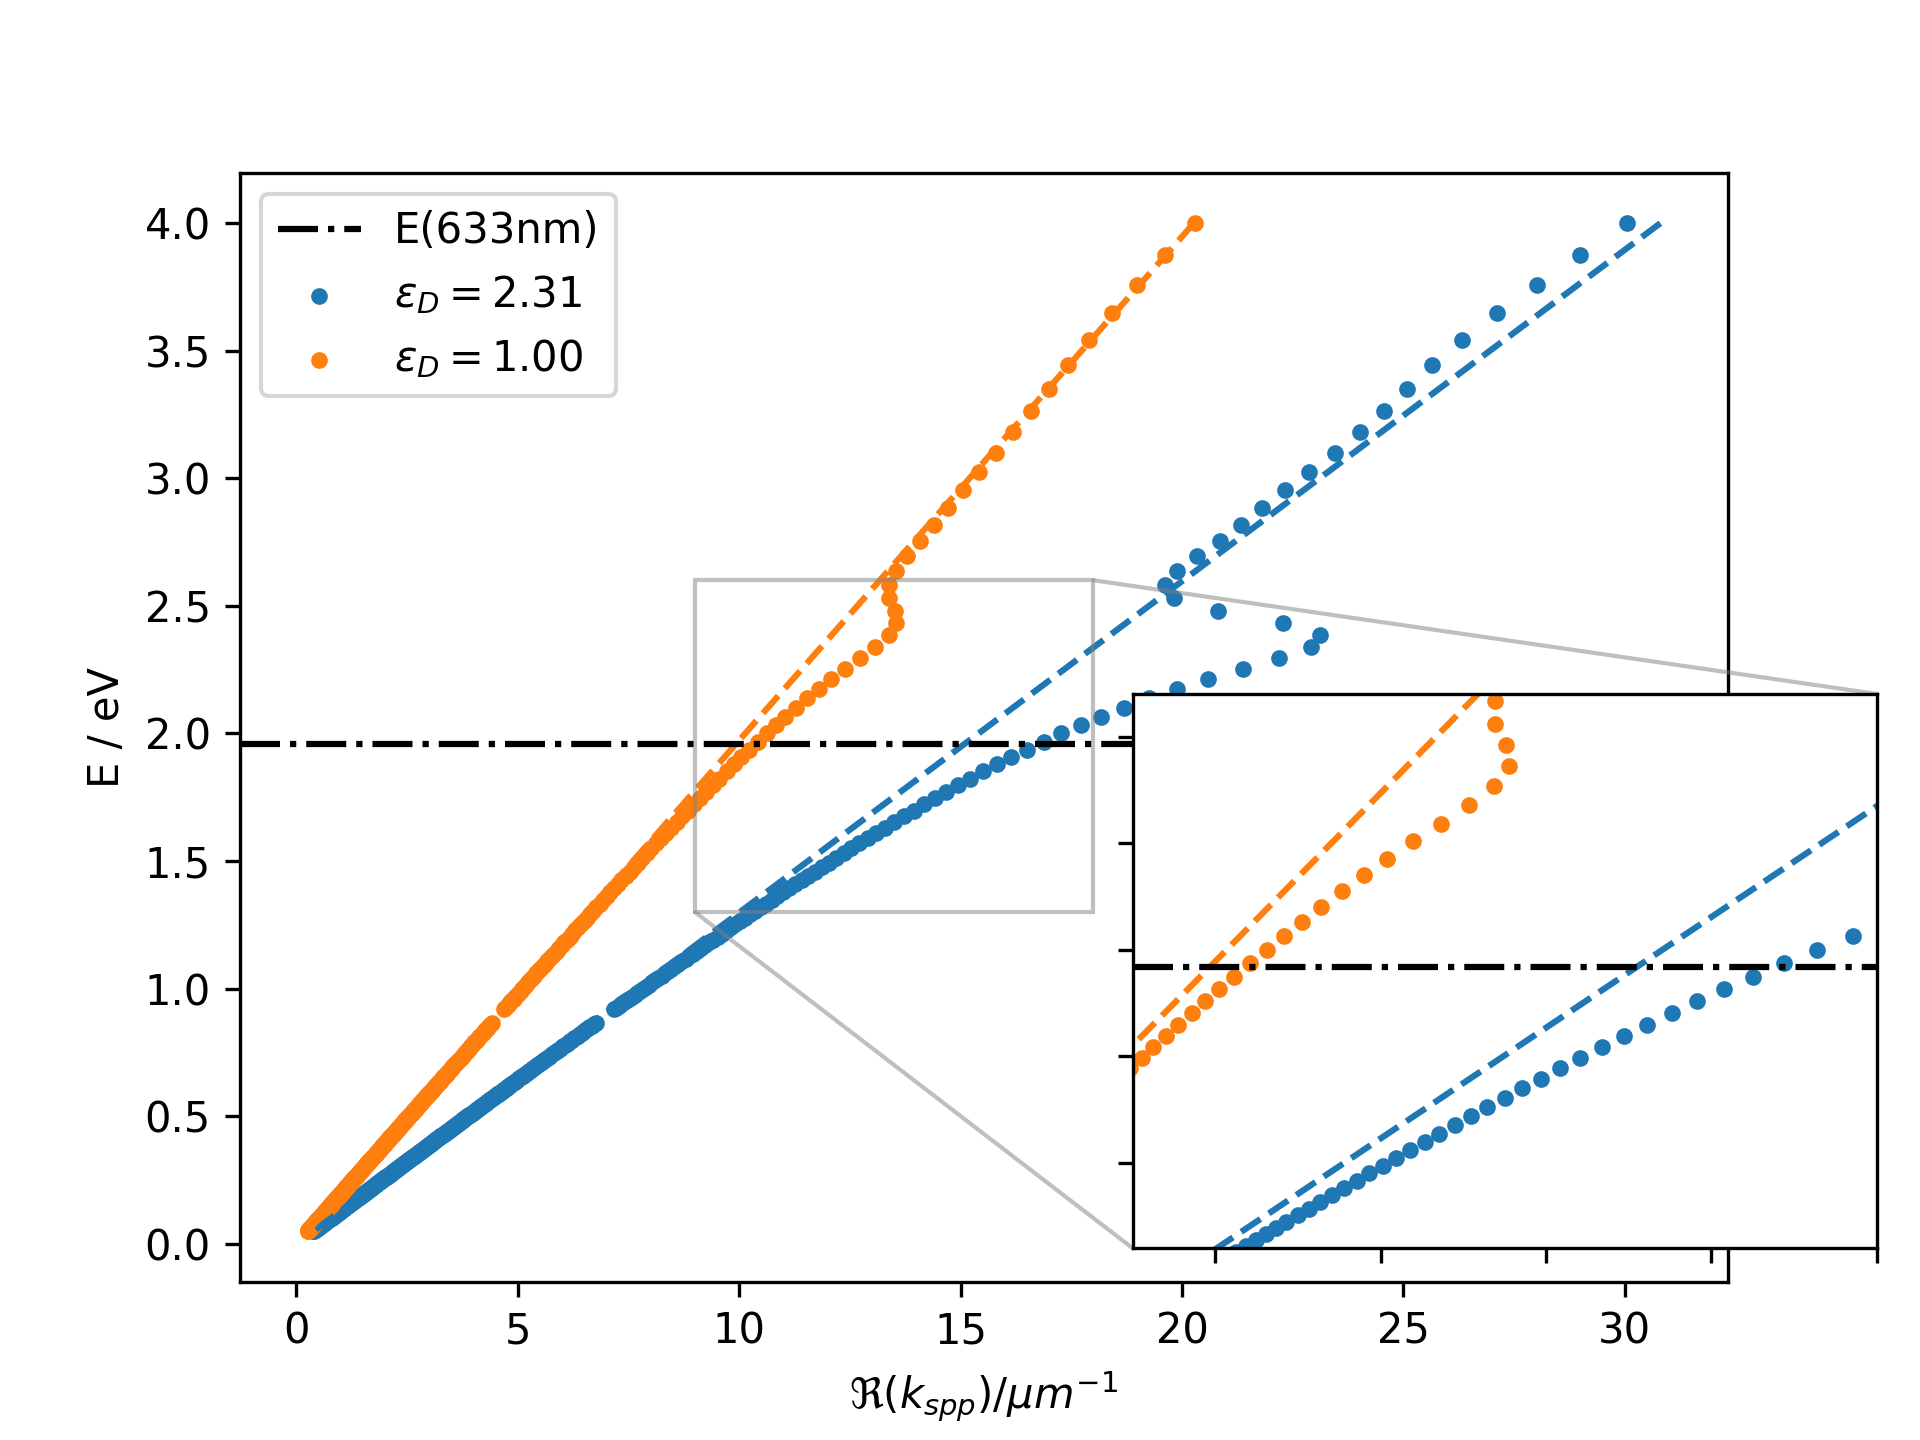
\includegraphics[width=1\textwidth]{figures/dispersion.png}
		\caption{Dispersionskurve der Gold-Vakuum und der Gold-Glas Mode. Do Lichtlinien im jeweiligen Medium sind zur Orientierung gestrichelt gekennzeichnet}		
	\end{figure}
	
		\subsubsection{Anregung}
			\paragraph{Kretschman-Konfiguration}
			\paragraph{Defekt-Anregung}
		\subsubsection{Leckstrahlung}
	\subsection{Plasmonischer-Spin-Hall-Effekt}r
	\subsubsection{Spin SPP, Photon}
		\paragraph{Transversal-Spin SPP}
		\paragraph{Longitudinal-Spin Photon}
	\subsubsection{Nahfeld zirkular-polarisierter Dipol}
	\subsection{Gerichtete Anregung durch anisotropes Nahfeld}	
\section{Messung und Methoden}
\subsection{Polarimeter, Verzögerungsplatte, Lineare Dichroismus}
	\subsubsection{Dichroismus}
	\subsubsection{Doppelbrechung}
	\subsubsection{Jones-Formalismus}
\subsection{Leckstrahlmikroskopie}
	\subsubsection{Immersionsobjektiv}
	\subsubsection{Fourier-Optik}
\subsection{Optischer Aufbau}
\subsection{Probe}
\subsection{Justage und Kalibrierung}
\section{Ergebnisse und Diskussion}
	\subsection{Bestimmung des Polarisationszustandes}
		\subsubsection{Modellierung Jones-Polarimeter}
		\subsubsection{least-square-fit}
	\subsection{Bestimmung des Kontrastverhältnisses linkes/rechtes SPP}
	\subsection{Diskussion}
	\begin{figure}[htbp] 
		\centering
		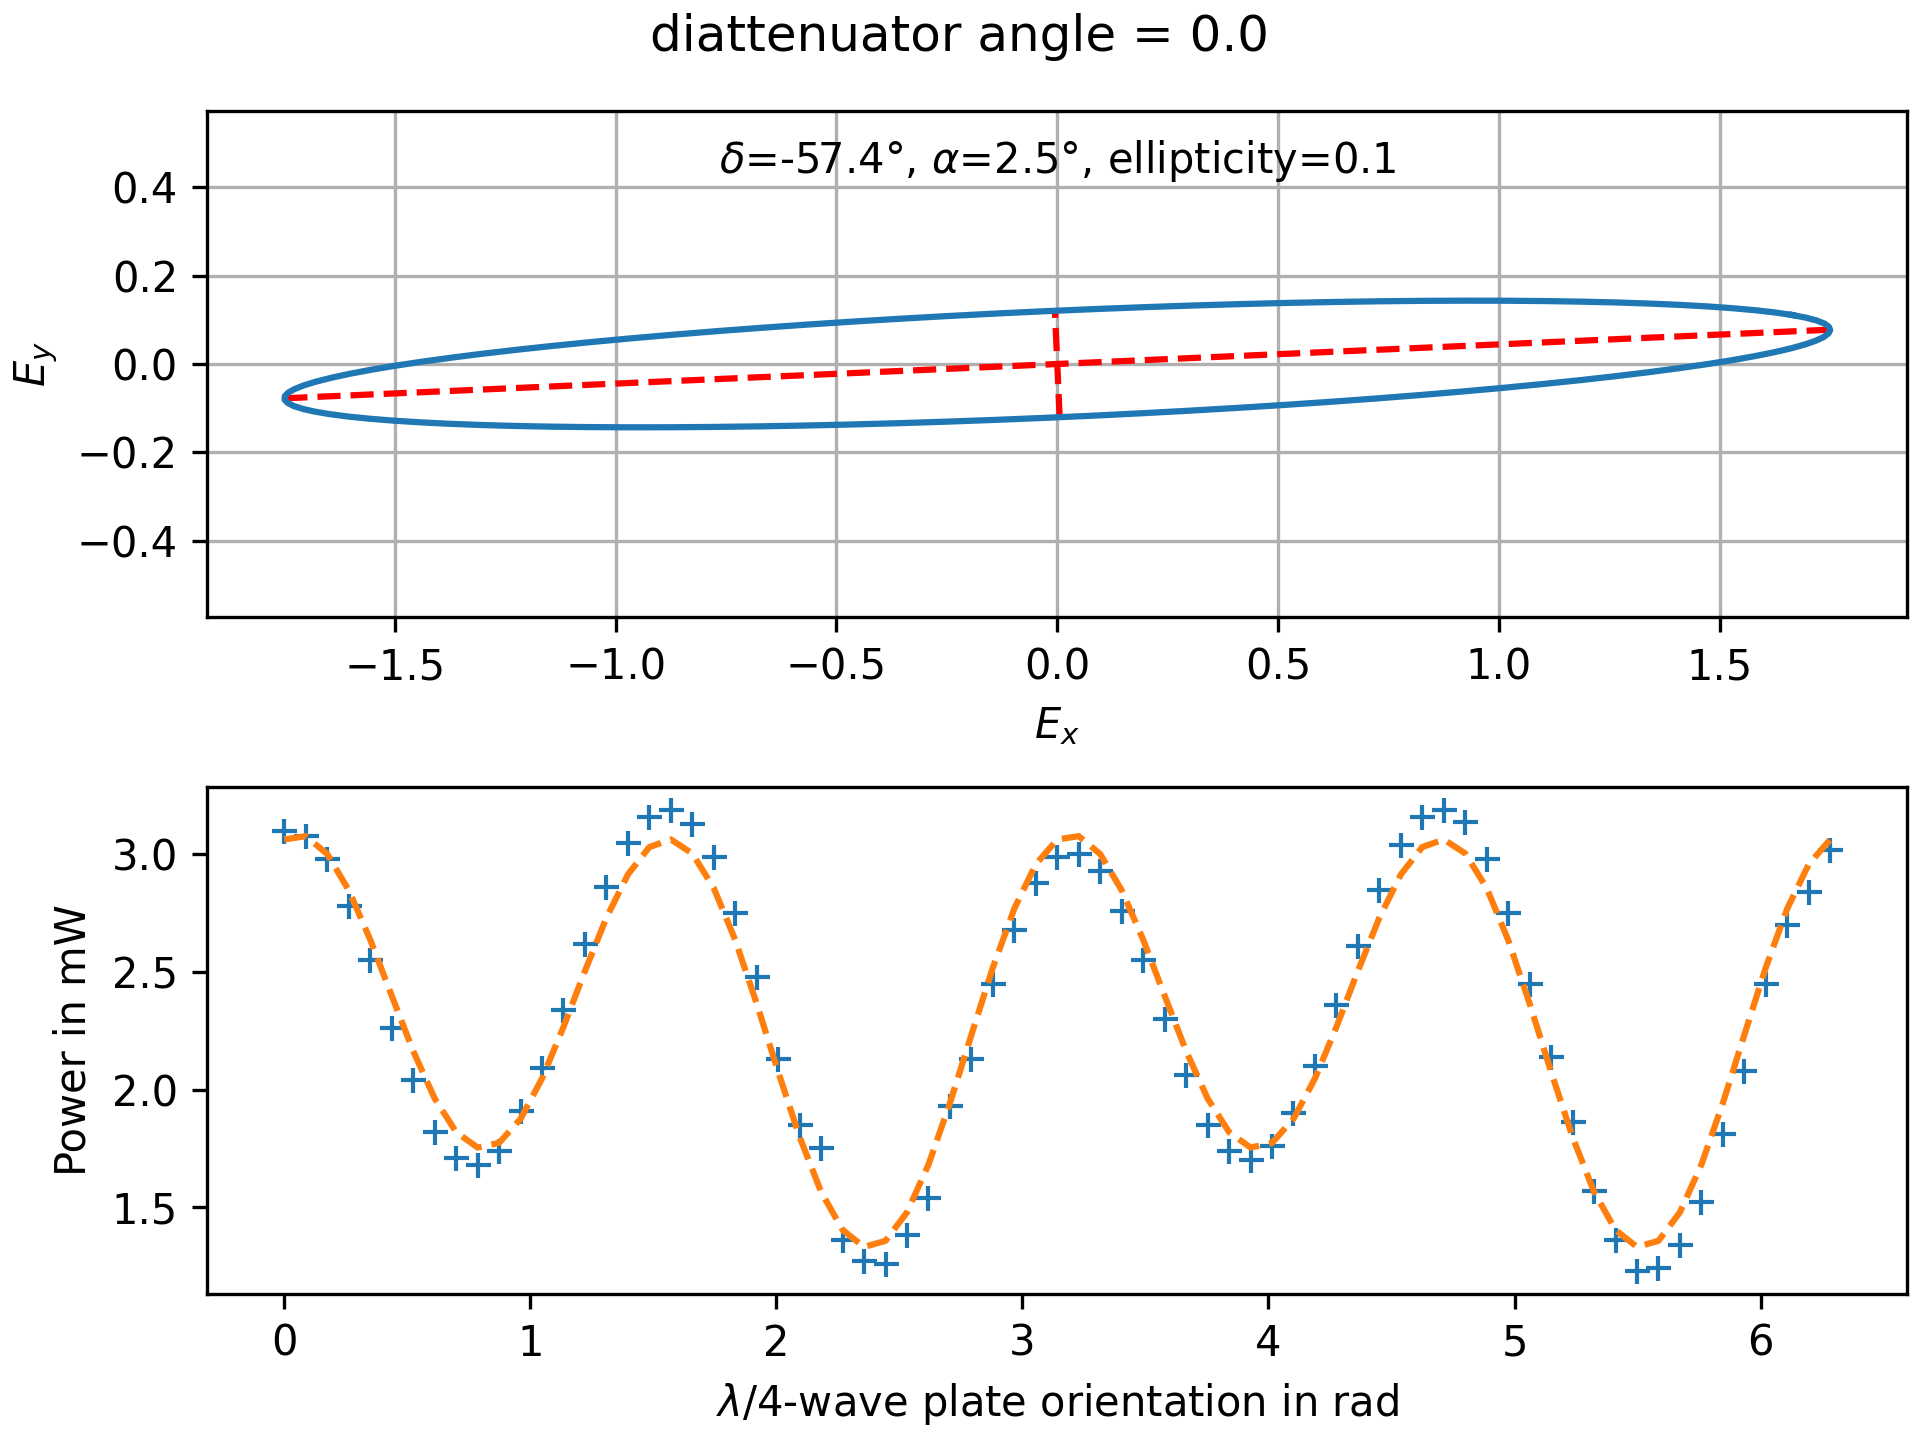
\includegraphics[width=0.7\textwidth]{figures/polarimeter.png}
		\caption{Polarisation}
		\label{fig:polarimeter}
	\end{figure}
\section{Zusammenfassung und Ausblick}
\newpage
\bibliography{bib}
	
\end{document}